\documentclass[border=3pt]{standalone}
% Preâmbulo compartilhado pelos diagramas TikZ da aula 14 (SLAM com EIF)
\usepackage[T1]{fontenc}
\usepackage[utf8]{inputenc}
\usepackage{lmodern}
\usepackage{amsmath}
\usepackage{xcolor}
\usepackage{tikz}
\usetikzlibrary{arrows.meta,angles,quotes,decorations.pathmorphing,decorations.pathreplacing,calc,
                positioning,shapes.geometric,shapes.misc,backgrounds,fit,
                math}

% Paleta (mesma dos SVGs originais)
\definecolor{dblue}{HTML}{2A5B8C}
\definecolor{dorange}{HTML}{B3541E}
\definecolor{dgreen}{HTML}{4A7C59}
\definecolor{dred}{HTML}{9C4B4B}
\definecolor{dcream}{HTML}{F4F1EA}
\definecolor{dshade}{HTML}{DDD7C9}

% Função gaussiana (não normalizada por padrão de escala visual)
\pgfmathdeclarefunction{gauss}{3}{%
  \pgfmathparse{1/(#3*sqrt(2*pi))*exp(-((#1-#2)^2)/(2*#3^2))}%
}

% Estilos comuns (prefixo d... para não colidir com chaves internas do pgf)
\tikzset{
  >={Stealth[length=2mm]},
  dguide/.style={gray!55, dashed, line width=0.4pt},
  daxis/.style={gray!60, line width=0.7pt, ->},
  dbody/.style={fill=black!3, draw=black!80, line width=1pt},
  dacc/.style={draw=dblue, line width=1pt},
  dlbl/.style={black!55, font=\small},
  dsub/.style={black!45, font=\footnotesize},
  dstate/.style={circle, draw=black!80, fill=dcream, line width=1pt,
                 minimum size=17mm, font=\large, inner sep=1pt},
  dobs/.style={circle, draw=black!80, fill=dshade, line width=1pt,
               minimum size=14mm, font=\large, inner sep=1pt},
  dbox/.style={rounded corners=2pt, draw=black!80, fill=dcream, line width=1pt,
               align=center, inner sep=6pt},
  dop/.style={circle, draw=black!80, fill=white, line width=1pt,
              minimum size=6mm, inner sep=0pt, font=\small},
  dtrans/.style={->, dblue, line width=1pt},
  dmeas/.style={->, dorange, line width=1pt},
  dcurve/.style={line width=1pt, dblue},
  dcurveb/.style={line width=1.4pt, dorange},
}

\begin{document}
\hyphenpenalty=10000 \exhyphenpenalty=10000 \tolerance=9999 \emergencystretch=3em
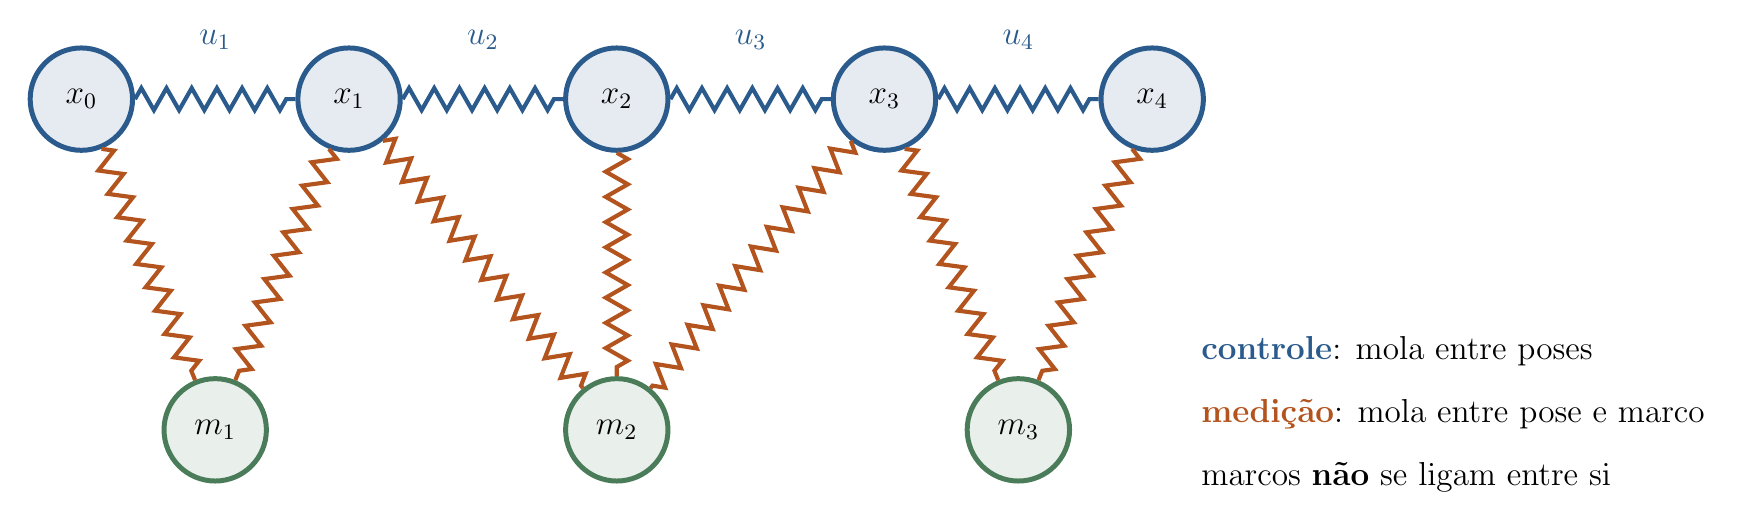
\begin{tikzpicture}[x=1cm,y=1cm]
\tikzset{p/.style={circle, draw=dblue, fill=dblue!12, line width=1.8pt, minimum size=1.3cm, font=\large},
        m/.style={circle, draw=dgreen, fill=dgreen!12, line width=1.8pt, minimum size=1.3cm, font=\large},
        sp/.style={decorate, decoration={zigzag, segment length=3.2mm, amplitude=1.4mm}, line width=1.5pt}}
\foreach \i in {0,1,2,3,4} {\node[p] (x\i) at ({1.4+\i*3.4},6.0) {$x_{\i}$};}
\foreach \i/\j in {0/1,1/2,2/3,3/4} {\draw[sp, draw=dblue] (x\i) -- (x\j);}
\foreach \i/\j in {0/1,1/2,2/3,3/4} {\node[font=\large, text=dblue, fill=white, inner sep=1pt] at ({1.4+\i*3.4+1.7},6.75) {$u_{\j}$};}
\node[m] (m1) at (3.1,1.8) {$m_1$};
\node[m] (m2) at (8.2,1.8) {$m_2$};
\node[m] (m3) at (13.3,1.8) {$m_3$};
\draw[sp, draw=dorange] (x0) -- (m1); \draw[sp, draw=dorange] (x1) -- (m1);
\draw[sp, draw=dorange] (x1) -- (m2); \draw[sp, draw=dorange] (x2) -- (m2); \draw[sp, draw=dorange] (x3) -- (m2);
\draw[sp, draw=dorange] (x3) -- (m3); \draw[sp, draw=dorange] (x4) -- (m3);
\node[font=\large, anchor=west] at (15.5,2.8) {\textcolor{dblue}{\textbf{controle}}: mola entre poses};
\node[font=\large, anchor=west] at (15.5,2.0) {\textcolor{dorange}{\textbf{medição}}: mola entre pose e marco};
\node[font=\large, anchor=west] at (15.5,1.2) {marcos \textbf{não} se ligam entre si};
\end{tikzpicture}
\end{document}
